\chapter{初识操作系统}

\section{实验目的}
  \begin{enumerate}
    \item 认识操作系统实验环境
    \item 掌握操作系统实验所需的基本工具
  \end{enumerate}
  
在本章中,我们需要去了解实验环境,熟悉Linux 操作系统(Ubuntu),了解控制终端,掌握一些常用工具并能够脱离可视化界面进行工作。本章节难度非常低,旨在让大家熟悉操作系统实验环境的各类工具,为后续实验奠定基础。

\section{初识实验}
所谓工欲善其事必先利其器,我们需要对我们的环境和工具有了足够多的了解才能开始我们的工作,本章内容看似简单,但实则不可忽略,请大家认真对待。
对于课程设计这名称,大家上次接触是《计算机组成课程设计》,也相信这门课程为大家带来了一段难忘而珍贵的记忆。就像“计组”一样,我们的课程也需要如ISE这样的开发环境,但好消息是,我们的环境约束要少得多,那么接下来熟悉一下我们的实验环境。

\subsection{了解实验环境}
实验环境整体配置如下:
	操作系统:Linux虚拟机,Ubuntu 12.04.5 LTS
	硬件模拟器:Gxemul
	编译器:GCC
	版本控制:Git
Ubuntu,版本号为12.04.5 LTS。Ubuntu是一款开源的GNU/Linux操作系统,基于Linux内核实现,是目前较为流行的几个Linux发行版之一。GNU (GNU is Not Unix的递归缩写),是一套计划,其中包含了三个协议条款,为我们带来了大量开源软件;Linux:严格意义上指代Linux内核,基于该内核的操作系统众多,具有免费、可靠、安全、稳定、多平台等特点。

GXemul,一款计算机架构仿真器,可以模拟所需硬件环境,例如我们需要的MIPS架构下的CPU。

GCC,一套免费、开源的编译器,诞生并服务于GNU计划,最初名称为GNU C Compiler,后支持了更多编程语言而改名为GNU Compiler Collection,如你所见,简称没变,很多我们熟知的IDE/集成开发环境的编译器用的便是GCC套件,例如Dev-C++,Code::Blocks等。我们的实验将使用mips-C交叉编译器。

Git,一款免费、开源的版本控制系统,我们的实验将用它为大家提供管理、发布、提交、评测等功能。0.5小节将会为大家详细介绍Git为何物以及如何使用,故不在此赘述。

\begin{figure}[htbp]
  \centering
  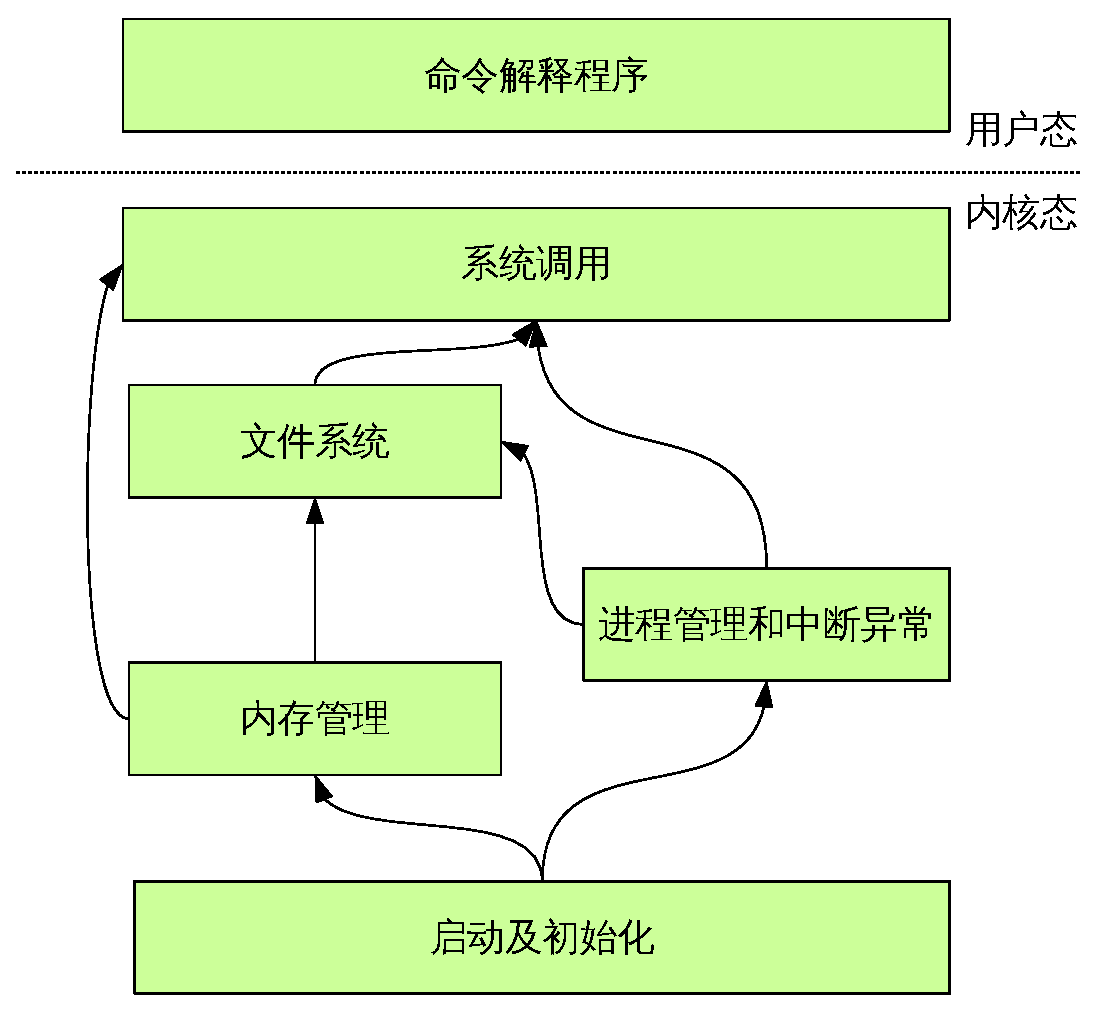
\includegraphics[height=4cm]{0-1}
  \caption{Ubuntu,GNU,Linux}\label{fig:0-1}
\end{figure}

\subsection{ssh—远程访问我们的环境}

熟悉了实验环境之后,我们不禁产生了疑问:难道这些环境全部需要我们自行安装和配置?这里为大家带来另一个好消息:当然不是,这些环境已经为你们配置好了!

本实验总计7个Lab完全依赖于远程的一台虚拟机上,最终成果也需要通过这台机器进行提交,所以同学们几乎不用担心个人电脑“带不动”实验环境,你需要的仅仅是一个能够支持ssh协议的远程连接工具。

一般Liunx或Mac OS等类Unix操作系统都会附带ssh客户端,即直接在终端使用ssh命令便可,Windows平台一般不自带ssh,需要下载第三方软件,在这里建议大家使用一款轻量级的,开源的,名为PuTTY的小工具,当然也不乏各种功能强大的工具,接触过git for Windows或对Windows 10有所研究的同学亦可使用git bash的以及Windows 10的几款Linux子系统。

在Host Name部分填入username@ip便可,username为同学们的学号,ip会在课上公布,之后单击open便可

在光标处输入密码便可,密码初始为同学们的学号,因此建议登录后立刻使用passwd命令更改密码,详细操作会在第三节中介绍。

如果同学们是在Mac OS的终端或Linux系统的终端,只需输入 ssh username@ip 之后的操作与PuTTY便相同了。

\begin{minted}[linenos]{bash}
# username 处填写你的用户名,ip处填写远程主机的地址
$ ssh username@ip
# 之后等候片刻会要求你输入密码,输入的密码不会被显示在屏幕上,输入完成后按回车即可
# 链接后会显示一些欢迎信息,下面是欢迎信息的一个例子
Welcome to Ubuntu 12.04.5 LTS (GNU/Linux 3.13.0-32-generic i686)

 * Documentation:  https://help.ubuntu.com/

  System information as of Tue Aug 11 09:55:40 CST 2015
  System load:  0.0                Processes:           118
  Usage of /:   8.7% of 145.55GB   Users logged in:     0
  Memory usage: 6%                 IP address for eth0: 0.0.0.0
  Swap usage:   0%

  Graph this data and manage this system at:
    https://landscape.canonical.com/

0 packages can be updated.
0 updates are security updates.
# 欢迎信息后会出现命令提示符,等待你输入命令。
\end{minted}

\begin{figure}[htbp]
  \centering
  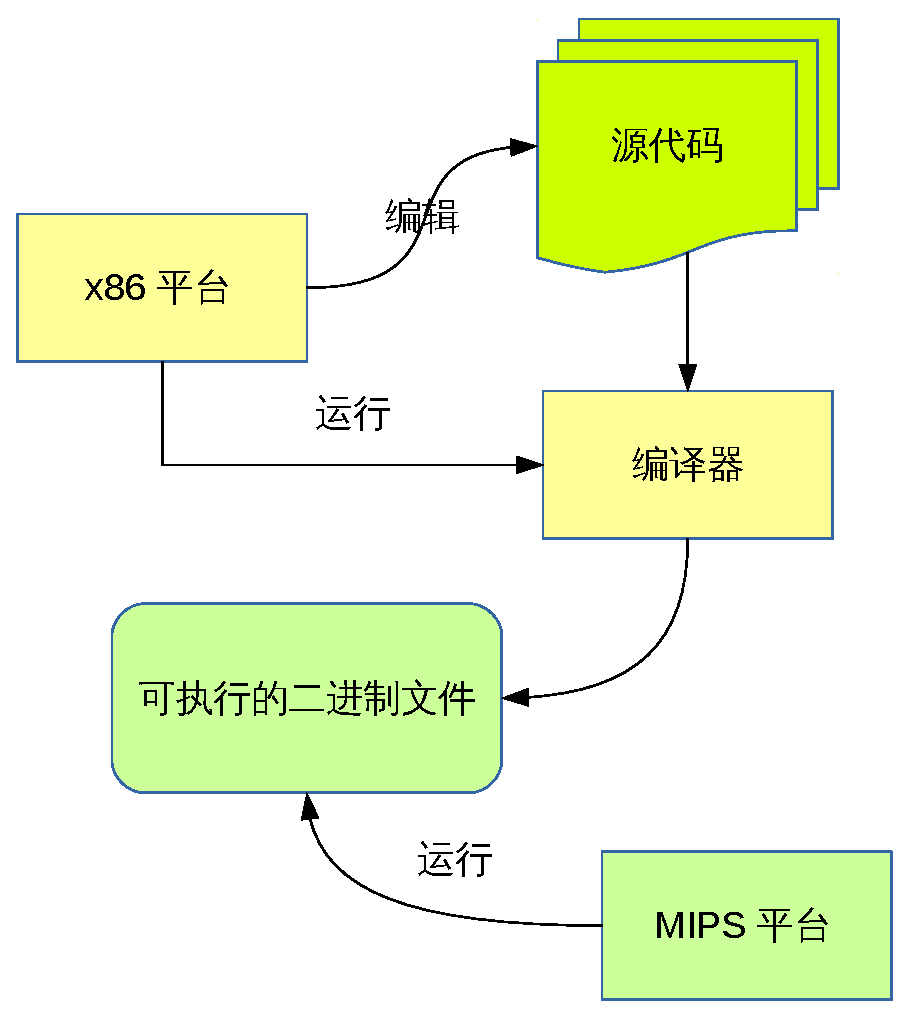
\includegraphics[height=8cm]{0-2}
  \caption{PuTTY登录界面}\label{fig:0-2}
\end{figure}

\begin{note}
SSH是Secure Shell的缩写。它是一种用于建立安全的远程连接的网络协议。在Unix类系统上被广泛采用。
除了连接到远程网络,目前SSH还有一种较为有趣的用法。当你既想用Windows,又有时需要Unix环境时,
可以利用Windows8及以上版本自带的Hyper-V开启一个Linux虚拟机(不必开启图形界面)。
之后通过SSH客户端连接到本机上的Linux虚拟机上,即可获得一个Unix环境。甚至可以开启X11转发,
即可在Windows上开启一些Linux上的带图形界面的程序,十分方便。
\end{note}

\subsection{接触CLI Shell,告别GUI Shell}

当你使用如上方法登录了自己的账号后,可能会有点不知所措并产生疑问:在我面前的这些东西是什么?

简单来说,这就是你们要接触的操作系统Ubuntu,在这里为从未使用过命令行的同学们解释一下,当你阅读这份文档时,你所使用的一定是一款拥有图形化界面的操作系统,一般来讲是Windows、Mac OS、Ubuntu等,而你面前的这个黑黑的东西就是一个没有图形化界面的操作系统,也就是模拟终端,我们为什么剥夺了你使用图形化界面的权力呢,原因有二:1.为了锻炼同学们在相对图形化恶劣的环境下工作的能力;2.你们的任务通过终端全部可以实现。

当然上文的描述是不严谨的,你所面对的并不是真正的“Ubuntu操作系统”,而是它的“壳”。一般的,我们管操作系统核心部分称为内核(英文:Kernel),与其相对的就是它最外层的壳(英文:Shell)。Shell是用于访问操作系统服务的用户界面。一般而言,操作系统shell使用命令行界面(CLI)或图形用户界面(GUI),这个纯文本的界面就是命令行界面,它能接收你发送的命令,如果命令存在于环境中,它便会为你提供相应的功能。

在Ubuntu中,我们默认使用的CLI shell是bash,也是一款基于GNU的免费、开源软件,那么接下来我们小试牛刀。

\begin{exercise}
在bash中分别输入
  \begin{itemize}
    \item echo “Hello Ubuntu”
    \item bash --version
    \item ls
  \end{itemize}
三条命令,简单思考其回显结果
\end{exercise}

可以保证的是,当你掌握了本章的知识后,再使用这款未为你准备图形化界面的操作系统时,将会得心应手,相信你能发挥出它本真的功能。

\begin{thinking}\label{think-Shell简析}
通过你的使用经验,简单分析CLI Shell,GUI Shell在你使用过程中的各自优劣(100字以内)
\end{thinking}

\subsection{获取实验包}

当我们登陆了课程实验环境后,就要准备开始我们的实验了,好奇的你可能会问:环境有了,工具有了,我们在哪里完成实验呢?

我们在ip服务器上为所有同学部署了实验的远程仓库,接下来我们要先进行一条命令来获取我们的实验包。
\begin{minted}[linenos]{bash}
$ git clone git@ip:id-lab
\end{minted}
接下来系统会提示如下内容
\begin{minted}[linenos]{bash}
Cloning into '16xxxxxx-lab'...
Enter passphrase for key '/home/16xxxxxx/.ssh/id_rsa':
\end{minted}
这里让你输入你的rsa密钥,也就是每个人的学号。

执行之后若输入ls,你会发现你的主目录下多了一个id-lab,输入如下命令访问它
\begin{minted}[linenos]{bash}
$ cd id-lab
\end{minted}
再使用ls会发现里面空空如也,不用着急,接下来需要再执行一条命令
\begin{minted}[linenos]{bash}
$ git checkout lab0
\end{minted}
这样我们就进入Lab0工作区了,也许你现在对上面的几条命令的功能不太了解,没关系,本章的后续内容会为你介绍它们。

\section{基础操作介绍}
\subsection{命令行}
走到这里,我们要正式与那黑黑的界面交流了,命令行界面(Command Line Interface,简称CLI)中,用户或客户端通过单条或连续命令行的形式向程序发出命令,从而达到与计算机程序进行人机交互的目的。在Linux系统中,命令即是对Linux系统进行管理的一系列命令,其一般格式为:命令名 [选项] [参数],其中中括号表示可选,意为可有可无(例如: ls –a directory)。对于Linux系统来说,无论是中央处理器、内存、磁盘驱动器、键盘、鼠标,还是用户等都是文件,Linux系统的管理命令是它正常运行的核心,与Windows的命令提示符(CMD)命令类似。Linux命令在系统中有两种类型:内置Shell(外壳)命令和Linux命令。

对于刚接触到命令行界面的各位萌新们来说,因为不清楚基本的Linux命令而呆呆地望着屏幕上的光标,想要做些什么却又不知所措是再正常不过的事。不过不要着急,万事开头难,学会并可以熟练使用下面介绍的一些基本操作之后,相信你们一定会对命令行界面有一个全新的认识,不再一头雾水。

\subsection{Linux基本操作命令}
通过SSH连接服务器打开Linux命令行界面后,首先会看到光标前的如下内容,其中@符号前的是用户名,@符号后的是计算机名,冒号后为当前所在的文件目录(/表示根目录root;~表示主目录home,其一般等价于/home/<user\_name>),最后的\$或\#分别表示当前用户为普通用户或超级用户root,当然,我们的服务器自然不会让大家知道root的密码的,感兴趣的同学可以自己配置系统娱乐一番

\begin{minted}[linenos]{bash}
16xxxxxx@ubuntu:~$
\end{minted}
\begin{minted}[linenos]{bash}
root@ubuntu:~#
\end{minted}

现在通过键盘输入命令,按回车后即可执行。首先,我们需要更改自己的用户密码,使用passwd命令即可更改当前用户的密码,注意:输入密码时不会在屏幕上显示密码内容(若输入过程中手抖打错,可重复多按几次退格键清空之前的输入后重新输入)。

\begin{minted}[linenos]{bash}
16xxxxxx@ubuntu:~$ passwd
更改16xxxxxx的密码。
(当前)UNIX密码:
输入新的UNIX密码:
重新输入新的UNIX密码:
passwd:已成功更新密码
\end{minted}

更改完密码后我们就可以安全的使用此用户来完成工作了,面对一个全新的界面,我们首先要知道当前目录中都有哪些文件,这时就需要使用ls命令,其输出信息可以进行彩色加亮显示,以分区不同类型的文件,是使用率较高的命令,其详细信息如下图所示。一般情况下,该命令的参数省略则默认显示该目录下所有文件,所以我们只需使用ls即可看到所有非隐藏文件,若要看到隐藏文件则需要加上-a选项,若要查看文件的详细信息则需要加上-l选项。

\begin{minted}[linenos]{bash}
ls - list directory contents
用法:ls [选项]... [文件]...
选项(常用):
		-a		不隐藏任何以. 开始的项目
		-l		每行只列出一个文件
\end{minted}

\begin{note}
与ls命令类似的目录查看命令还有tree命令,它可以根据文件目录生成文件树,这个命令就交给大家自己去实践吧。
\end{note}

然后你就会发现主目录中空空如也,又不知道要做什么好了,这时我们可以使用mkdir命令创建文件目录(即Windows系统中的文件夹),该命令的参数为创建的新目录的名称,如:mkdir newdir 为创建一个名为newdir的目录。

\begin{minted}[linenos]{bash}
mkdir - make directories
用法:mkdir [选项]... 目录...
\end{minted}

删除空目录的命令rmdir与其类似,其命令参数为需要删除的空目录的名称,这里要注意只有空目录才可以使用rmdir命令删除。

\begin{minted}[linenos]{bash}
rmdir - remove empty directories
用法:rmdir [选项]... 目录...
\end{minted}

那么目录非空时怎么办呢?这就需要用到搞破坏者最喜欢的rm命令了,rm命令可以删除一个目录中的一个或多个文件或目录,也可以将某个目录及其下属的所有文件及其子目录均删除掉。对于链接文件,只是删除整个链接文件,而原有文件保持不变。

\begin{minted}[linenos]{bash}
rm - remove files or directories
用法:rm [选项]... 文件...
选项(常用):
		-r		递归删除目录及其内容
		-f		强制删除。忽略不存在的文件,不提示确认
\end{minted}

\begin{note}
使用rm命令要格外小心,因为一旦删除了一个文件,就无法再恢复它。所以,在删除文件之前,最好再看一下文件的内容,确定是否真要删除。
\end{note}

此外,rm命令可以用-i选项,这个选项在使用文件扩展名字符删除多个文件时特别有用。使用这个选项,系统会要求你逐一确定是否要删除。这时,必须输入y并按Enter键,才能删除文件。如果仅按Enter键或其他字符,文件不会被删除。与之相对应的就是-f选项,强制删除文件或目录,不询问用户。使用该选项配合-r选项,进行递归强制删除,强制将指定目录下的所有文件与子目录一并删除可以达到毁灭性效果。例如:rm –rf / 即可强制递归删除全盘文件,有兴趣的同学可以尝试一下,反正你们也没有这个权限~

\begin{note}
在需要键入文件名/目录名时,可以使用TAB键补足全名,当有多种补足可能时双击TAB键可以显示所有可能选项。
\end{note}

学会创建目录后,我们就需要进入我们新建的目录中创建和修改文件来完成工作了。使用cd命令来切换工作目录至dirname,其中dirname的表示法可为绝对路径或相对路径。若目录名称省略,则变换至使用者的主目录home (等价于cd ~ )。另外,在Linux文件系统中,"."表示当前所在目录,".."表示当前目录位置的上一层目录,同学们在使用ls –a后看到的目录中的"."和".."即使如此。

\begin{minted}[linenos]{bash}
cd - change working directory
用法:cd [路径]
e.g.
		cd .	变更至当前目录
		cd ..	变更至父目录
\end{minted}

现在,进入新建的目录中后依旧空空如也,那么我们就来创建几个文件玩玩~创建文件的方法有很多,可以直接使用重定向输出>filename来新建一个空文件,也可以使用文本编辑工具vim或nano等新建文件后保存(使用命令vim filename或nano filename,编辑工具的使用方法将在0.4节介绍),因为打开后可以直接进行编辑后保存,所以笔者更喜欢用后者新建文件。现在可能有人要问了,重定向输出是什么意思?大于号是什么意思?重定向输出就是使用>来改变送出的数据信道,使>前命令的输出数据输出到>后指定的文件中去。例如:ls / > filename 可以将根目录下的文件名输出至当前目录下的filename文件中。与之类似的,还有重定向追加输出>>,将>>前命令的输出数据追加输出到>>后指定的文件中去;以及重定向输入<,将<后指定的文件中的数据输入到<前的命令中,同学们可以自己动手实践一下。

在此顺带一提echo命令,echo命令用于在Shell中打印Shell变量的值,或者直接输出指定的字符串。简单来说,就是将echo命令中的参数输出到屏幕上显示。那么将echo命令和重定向相结合会产生什么样的效果呢?这就留给大家自己去尝试吧~

好了,现在我们已经创建了新的文件,那么想要查看文件内容要怎么办呢?除了前面说到的编辑工具以外,还有一种简单快速查看文件内容的方法——cat命令。使用cat filename即可将文件内容输出到屏幕上显示,若要显示行数,添加-n选项即可。

\begin{minted}[linenos]{bash}
cat - concatenate files and print
用法:cat [选项]... [文件]...
选项(常用):
		-n		对输出的所有行编号
\end{minted}

\begin{exercise}
	执行如下命令,并查看结果
	\begin{itemize}
		\item echo first
		\item echo second > output.txt
		\item echo third > output.txt
		\item echo forth >> output.txt
	\end{itemize}
\end{exercise}
之后就是对于文件的操作:复制和移动。复制命令为cp,命令的第一个参数为源文件路径,命令的第二个参数为目标文件路径。

\begin{minted}[linenos]{bash}
cp - copy files and directories
用法:cp [选项]... 源文件... 目录
选项(常用):
		-r		递归复制目录及其子目录内的所有内容
\end{minted}

移动命令为mv,与cp的操作相似。例如:mv file ../file\_mv就是将当前目录中的file文件移动至上一层目录中且重命名为file\_mv。聪明的你应该已经看出来,在Linux系统中想要对文件进行重命名操作,使用mv oldname newname命令就可以了。
\begin{minted}[linenos]{bash}
mv - move/rename file
用法:mv [选项]... 源文件... 目录
\end{minted}

在以后的工作中,可能会遇到重复多次用到单条或多条长而复杂命令的情况,初学者可能会想把这些命令保存在一个文件中,以后再打开文件复制粘贴运行,其实大可不必复制粘贴,将文件按照批处理脚本运行即可。简单来说,批处理脚本就是存储了一条或多条命令的文本文件,Linux系统中有一种简单快速执行批处理文件的方法(类似Windows系统中的.bat批处理脚本)——source命令。source命令是bash的内置命令,该命令通常用点命令 . 来替代。这两个命令都以一个脚本为参数,该脚本将作为当前Shell的环境执行,不会启动一个新的子进程,所有在脚本中设置的变量将成为当前Shell的一部分。使用方法如下图所示,其命令格式与之前介绍的命令类似,请同学们自己动手举例尝试。

\begin{minted}[linenos]{bash}
source - execute commands in file
用法:source 文件名 [参数]
注:文件应为可执行文件,即为绿色
\end{minted}

\begin{thinking}\label{think-文件的操作}
使用你知道的方法(包括重定向)创建下图内容的文件(文件命名为test),将创建该文件的命令序列保存在command文件中,并将test文件作为批处理文件运行,将运行结果输出至result文件中。给出command文件和result文件的内容,并对最后的结果进行解释说明(可以从test文件的内容入手)
\end{thinking}
\begin{figure}[htbp]
	\centering
	\includegraphics[height=8cm]{0-15}
	\caption{文件内容}\label{fig:0-15}
\end{figure}

此外,还有两种常用的查找命令:find和grep

使用find命令并加上-name选项可以在当前目录下递归地查找符合参数所示文件名的文件,并将文件的路径输出至屏幕上。

\begin{minted}[linenos]{bash}
find - search for files in a directory hierarchy
用法:find -name 文件名
\end{minted}

grep是一种强大的文本搜索工具,它能使用正则表达式搜索文本,并把匹配的行打印出来。简单来说,grep命令可以从文件中查找包含pattern部分字符串的行,并将该文件的路径和该行输出至屏幕。当你需要在整个项目目录中查找某个函数名、变量名等特定文本的时候,grep 将是你手头一个强有力的工具。

\begin{minted}[linenos]{bash}
grep - print lines matching a pattern
用法:grep [选项]... PATTERN [FILE]...
选项(常用):
		-a		不忽略二进制数据进行搜索
		-i		忽略文件大小写差异
		-r		从文件夹递归查找
\end{minted}

以上,就是Linux系统入门级的部分常用操作命令以及这些命令的常用选项,如果想要查看这些命令的其他功能选项或者新命令的详尽说明,就需要使用Linux下的帮助命令——man命令,通过man指令可以查看Linux中的指令帮助、配置文件帮助和编程帮助等信息。

\begin{minted}[linenos]{bash}
man - manual
用法:man page
e.g.
	man ls
\end{minted}

最后,还有下面几个常用的快捷键介绍给同学们。
\begin{itemize}
    \item Ctrl+C	终止当前程序的执行
	\item Ctrl+Z	挂起当前程序
	\item Ctrl+D	终止输入(若正在使用Shell,则退出当前Shell)
	\item Ctrl+I	清屏
\end{itemize}

其中,Ctrl+Z挂起程序后会显示该程序挂起编号,若想要恢复该程序可以使用fg <编号>即可。对其他内容感兴趣的同学可以自行百度或用man命令看帮助手册进行学习和了解。

\begin{note}
在多数shell中,四个方向键也是有各自特定的功能的:←和→可以控制光标的位置,↑和↓可以切换最近使用过的命令
\end{note}

\section{实用工具介绍}
学会了Linux基本操作命令,我们就可以得心应手地使用命令行界面的Linux操作系统了,但是想要使用Linux系统完成工作,光靠命令行还远远不够。在开始动手阅读并修改代码之前,我们还需要掌握一些实用工具的使用方法。这里我们首先介绍两种常用的文本编辑器:nano和Vim。
\subsection{nano}
我们先从一个简易的工具入手:nano。nano的主界面如下图所示,所有基本的操作都被罗列在下面。nano 较为容易上手,但功能相对有限。如果你需要更为强大的功能,那么推荐去学习和使用Vim。

\begin{figure}[htbp]
  \centering
  \includegraphics[height=8.5cm]{0-20}
  \caption{Nano界面及基础介绍}\label{fig:0-20}
\end{figure}

\subsection{Vim}
Vim被誉为编辑器之神,是程序员为程序员设计的编辑器,编辑效率高,十分适合编辑代码,其界面如下图\ref{fig:0-21}所示。对于习惯了图形化界面文本编辑软件的同学们来说,刚接触Vim时一定会觉得非常不习惯非常不顺手,所以在这里给大家总结了一些常用的基本操作以助入门。同时,推荐给大家一篇质量极高的Vim教程——《简明Vim练级攻略》(\url{http://coolshell.cn/articles/5426.html/}),只需要十多分钟的阅读,你就可以掌握 Vim的所有基本操作。当然,想要完全掌握它需要相当长的时间去练习,而如果你只想把Vim当成记事本用的话,几分钟的学习足矣。其他的内容网上有太多太多的资料,随用随查即可。

\begin{figure}[htbp]
  \centering
  \includegraphics[height=11cm]{0-21}
  \caption{Vim界面及基础介绍}\label{fig:0-21}
\end{figure}

\subsection{GCC}
在没有IDE的情况下,使用GCC编译器是一种简单快捷生成可执行文件的途径,只需一行命令即可将C源文件编译成可执行文件。其常用的使用方法如下图\ref{fig:0-22}所示,同学们可以自己动手实践,写一些简单的C代码来编译运行。如果想要同时编译多个文件,可以直接用-o选项将多个文件进行编译连接:gcc testfun.c test.c -o test ,也可以先使用-c选项将每个文件单独编译成.o文件,再用-o选项将多个.o文件进行连接:gcc -c testfun.c -> gcc -c test.c -> gcc testfun.o test.o -o test ,两者等价。

\begin{figure}[htbp]
  \centering
  \includegraphics[height=8cm]{0-22}
  \caption{GCC编译器}\label{fig:0-22}
\end{figure}

\section{Git专栏--轻松维护和提交代码}
经过上面的一系列的学习之后,你刚刚伸了个懒腰,也许准备喝杯茶休息休息。但突然你意识到了一个问题:之前好像说,有一个叫做Git的东西能对我们的学习进行评测?我们的实验是通过git版本控制系统进行管理,那么接下来,在本章的最后,我们就来了解一下git相关的内容。
\subsection{Git是什么?}
说到Git是什么,我们就得考虑什么是版本控制,最原始的版本控制是纯手工的版本控制:修改文件,保存文件副本。有时候偷懒省事,保存副本时命名比较随意,时间长了就不知道哪个是新的,哪个是老的了,即使知道新旧,可能也不知道每个版本是什么内容,相对上一版作了什么修改了,当几个版本过去后,很可能就是下面的样子了:
\begin{figure}[htbp]
  \centering
  \includegraphics[height=6cm]{0-23}
  \caption{手工版本控制}\label{fig:0-23}
\end{figure}

当然,有些时候,我们不仅是一个人写文本,那些工程项目也往往不是由一个人负责。

分工,制定计划,埋头苦干,看起来一切井然有序,后来却只会让人蛋疼不已。本质原因在于每个人都会对项目的内容进行改动,结果最后有了这样一副情形:A把添加完功能的项目打包发给了B,然后自己继续添加功能。一天后,B把他修改后的项目包又发给了A,这时A就必须非常清楚发给B之后到他发回来的这段期间,自己究竟对哪里做了改动,然后还要进行合并,相当困难。

这时我们发现了一个无法避免的事实:如果每一次小小的改动,项目负责人之间都要相互通知,那么一些错误的改动将会令我们付出惨痛的代价:一个错误的改动要频繁在几方同时通知纠正。如果一次性改动了大幅度的内容,那么只有概览了项目的多数文件才能知道改动在哪,也才能合并劳动成果。项目只有10个文件时还好接受,如果是40个, 60个,80个呢。

于是就产生了需求,我们希望有一款软件:
\begin{itemize}
    \item 自动帮我记录每次文件的改动,而且最好是有后悔药的功能,改错了一个东西,我可以轻松撤销。
	\item 还得有多人协作编辑不费力的好处,有着简洁的指令与操作。
	\item 最好能像时光机一样穿越回以前,而且不但能穿越回去,还能在不满意的时候穿越回来!
	\item 如果想查看某次改动,只需要在软件里瞄一眼就可以。
\end{itemize}
那岂不是美滋滋~

版本控制系统就是这样一种神器的系统。而 Git,则是目前世界上最先进的分布式版本控制系统,没有之一。

Git是由Linux的缔造者Linus Torvalds创造,最开始也是用于管理自己的Linux开发过程。他对于Git的解释是:The stupid content tracker,傻瓜内容追踪器。Git一次本身也是个俚语,大概表示“混帐”。

\begin{note}
版本控制是一种记录若干文件内容变化, 以便将来查阅特定版本修订情况的系统。
\end{note}

\subsection{Git基础指引}
看过上面的小案例后,相信好奇心旺盛的各位已经对Git充满了兴趣。那么Git在实际应用中究竟是怎样的一个系统呢?别着急,我们慢慢来。

先从Git最基础的指令讲起,通过前几节的学习,接下来请进行如下操作:
\begin{enumerate}
    \item 创建一个名为learnGit的文件夹
    \item 进入learnGit目录
	\item 输入git init
	\item 用ls指令添加适当参数看看多了什么
\end{enumerate}
我们会发现,新建的目录下面多了一个叫.git的隐藏目录,这个目录就是我们的Git版本库,更多的被称为仓库(repository)。需要注意的是,\textbf{在我们的实验中是不会对.git文件夹进行任何直接操作的,所以不要轻易动这个文件夹中的任何文件}

在init执行完后,我们就拥有了一个仓库。我们建立的learnGit文件夹就是Git里的工作区。目前我们除了.git版本库目录以外空无一物。

\begin{note}
在我们的小操作系统实验中我们不需要使用到 git init 命令,每个人一开始就都有一个名为 16xxxxxx-lab 的版本库,包含了 lab0 的实验内容。
\end{note}
既然工作区里空荡荡的,那我们来为他加点料:
用你已知的方法在工作区中建立一个readme.txt,内容为“BUAA\_OSLAB”
当然这只是创建了一个文件而已,下面我们要将它添加至版本库,执行如下内容
\begin{minted}[linenos]{bash}
$ git add readme.txt
\end{minted}
注意,到这里还没有结束,你可能会想,那我既然都把 readme.txt 加入了,难道不是已经提交到版本库了吗?但事实就是这样,Git——同其他大多数版本控制系统一样,add之后需要再执行一次提交操作,提交操作的命令如下:
\begin{minted}[linenos]{bash}
$ git commit
\end{minted}
如果不带任何附加选修,执行后会弹出一个说明窗口,如下所示:
\begin{minted}[linenos]{bash}
GNU nano 2.2.6    文件: /home/13061193/13061193-lab/.git/COMMIT_EDITMSG              

Notes to test.
# 请为您的变更输入提交说明。以 '#' 开始的行将被忽略,而一个空的提交
# 说明将会终止提交。
# 位于分支 master
# 您的分支与上游分支 'origin/master' 一致。
#
# 要提交的变更:
#       修改:         readme.txt
#

                                 [ 已读取9 行 ]
^G 求助      ^O 写入      ^R 读档      ^Y 上页      ^K 剪切文字  ^C 游标位置
^X 离开      ^J 对齐      ^W 搜索      ^V 下页      ^U 还原剪切  ^T 拼写检查
\end{minted}
在上面里书写的 \textbf{Notes to test}. 是我们本次提交所附加的说明。

注意,弹出的窗口中我们\textbf{必须}得添加本次 commit 的说明,这意味着我们不能提交空白说明,否则我们的提交不会成功。而且在添加评论之后,可以按提示按键来成功保存。

\begin{note}
初学者一般不太重视 git commit 内容的有效性,总是使用无意义的字符串作为说明提交。但以后你可能就会发现自己写了一个自己看得懂,别人也能看得懂提交说明是多么庆幸。所以尽量让你的每次提交显得有意义,比如“fixedabug in ...” 这样的描述,顺便推荐一条命令:git commit --amend,这条命令可以重新书写你最后一次 commit 的说明。
\end{note}

可能这样的窗口提交方式比较繁琐,我们可以采用一种简洁的方式:
\begin{minted}[linenos]{bash}
$ git commit -m [comments]
\end{minted}
[comments]格式为\textbf{“评论内容”},上述的提交过程我们可以简化为下面一条指令
\begin{minted}[linenos]{bash}
$ git commit -m "Notes to test."
\end{minted}
如果我们提交之后看到类似的提示就说明我们提交成功了
\begin{minted}[linenos]{bash}
[master 955db52] Notes to test.
 1 file changed, 1 insertion(+), 1 deletion(-)
\end{minted}
从我们本次提交中我们可以得到以下信息,可能现在你还不能完全理解这些信息代表的意思,但是没关系,之后我们会讲解

\begin{itemize}
\item 本次提交的分支\label{分支}是 master
\item 本次提交的ID是 955db52
\item 提交说明是 Notes to test
\item 共有1个文件相比之前发生了变化:1行的添加与1行的删除行为
\end{itemize}

但是在我们实验中,第一次提交可不会这么一帆风顺,我们第一次提交往往会出现 下面的提示
\begin{minted}[linenos]{c}
*** Please tell me who you are.

Run

  git config --global user.email "you@example.com"
  git config --global user.name "Your Name"

# to set your account’s default identity.
# Omit --global to set the identity only in this repository.
\end{minted}

相信大家从第一句也能推测出,这是要求我们设置提交者身份的。我们设置身份有 什么作用呢?别急,等你设置成功了我们再详谈。

\begin{note}
从上面我们也知道了,我们可以用  

  git config -{}-global user.email “you@example.com”
  
  git config -{}-global user.name “Your Name“
  
这两条命令设置我们的名字和邮箱,在我们的实验中对这两个没有什么要求,大家随性设置就好,给个示例:

  git config -{}-global user.email “qianlxc@126.com”
  
  git config -{}-global user.name “Qian”
\end{note}

现在你已设置了提交者的信息,那么做一下这个小练习来快速上手 Git 的使用吧。

\begin{exercise}
\begin{itemize}
    \item 在/home/16xxxxxx/learnGit(已init)目录下创建一个名为README.txt的文件。这时使用 git status > Untracked.txt 。
	\item 在 README.txt 文件中随便写点什么,然后使用刚刚学到的 add 命令,再使用 git status > Stage.txt 。
	\item 之后使用上面学到的 Git 提交有关的知识把 README.txt 提交,并在提交说明里写入自己的学号。
	\item 使用 cat Untracked.txt 和 cat Stage.txt,对比一下两次的结果,体会一下README.txt 两次所处位置的不同。
	\item 修改 README.txt 文件,再使用 git status > Modified.txt 。
	\item 使用 cat Modified.txt ,观察它和第一次 add 之前的 status 一样吗,思考一 下为什么?
\end{itemize}
\end{exercise}

\begin{note}
git status 是一个查看当前文件状态的有效指令,而 git log 则是提交日志,每commit一次,Git 会在提交日志中记录一次。git log 将在我们后面乘坐时光机时发挥很大的作用。
\end{note}

相信你做过上述实验后,心里还是会有些疑惑,没关系,我们来一起看一下我们刚才得到的 Untracked.txt ,Stage.txt 和 Modified.txt 的内容
\begin{minted}[linenos]{bash}
Untracked.txt的内容如下

# On branch master
# Untracked files:
#   (use "git add <file>..." to include in what will be committed)
#
#	README.txt
nothing added to commit but untracked files present (use "git add" to track)

Stage.txt的内容如下

# On branch master
# Changes to be committed:
#   (use "git reset HEAD <file>..." to unstage)
#
#	new file:   README.txt
#

Modified.txt的内容如下

# On branch master
# Changes not staged for commit:
#   (use "git add <file>..." to update what will be committed)
#   (use "git checkout -- <file>..." to discard changes in working directory)
#
#	modified:   README.txt
#
no changes added to commit (use "git add" and/or "git commit -a")
\end{minted}
通过仔细观察,我们看到第一个文本文件中第 2 行是:Untracked files,而第二个文本文件中第二行内容是:Changes to be committed,而第三个则是 Changes not staged for commit。这三种不同的提示意味着什么,需要你通过后面的学习找到答案,答案就在不远处。

我们开始时已经介绍了 Git 中的工作区的概念,接下来的内容就是 Git 中的最核心的概念,为了能自如运用 Git 中的命令,你一定要仔细学习。

\subsection{Git文件状态}
首先对于任何一个文件, 在 Git 内都只有四种状态: 未跟踪 (untracked)、未修改 (unmodified)、已修改 (modified)、已暂存 (staged)
\begin{description}
\item[未跟踪] 表示没有跟踪(add)某个文件的变化,使用git add即可跟踪文件
\item[未修改] 表示某文件在跟踪后一直没有改动过或者改动已经被提交
\item[已修改] 表示修改了某个文件,但还没有加入(add)到暂存区中
\item[已暂存] 表示把已修改的文件放在下次提交(commit)时要保存的清单中
\end{description}

\begin{note}
关于刚才的 exercise 中的思考,实际上是因为 git add 指令本身是有多义性的,虽然差别较小但是不同情境下使用依然是有区别。我们现在只需要记住:新建文件后要 git add,修改文件后也需要 git add。
\end{note}

我们使用一张图来说明文件的四种状态的转换关系

\begin{figure}[htbp]
	\centering
	\includegraphics[width=9.5cm]{git-change}
	\caption{Git中的四种状态转换关系}\label{fig:git-change}
\end{figure}

\begin{thinking}\label{think-箭头与指令}
仔细看看这张图,思考一下红箭头里的 add the file 、stage the file 和commit 分别对应的是 Git 里的哪些命令呢?
\end{thinking}

看到这里,相信你对 Git 的设计有了初步的认识。下一步我们就来深入理解一下 Git 里的一些机制,从而让我们可以一次上手,终身难忘。

\subsection{Git三棵树}
我们的本地仓库由 git 维护的三棵“树”组成。第一个是我们的工作区,它持有实际文件;第二个是暂存区(Index 有时也称 Stage),它像个暂时存放的区域,临时保存你的改动;最后是 HEAD,指向你最近一次提交后的结果。 

在我们的.git 目录中,文件.git/index 实际上就是一个包含文件索引的目录树,像是一个虚拟的工作区。在这个虚拟工作区的目录树中,记录了文件名、文件的状态信息(时间戳、文件长度等),但是文件的内容并不存储其中,而是保存在 Git 对象库(.git/objects)中,文件索引建立了文件和对象库中对象实体之间的对应。下面这个图展示了工作区、版本库中的暂存区和版本库之间的关系,希望你能耐着性子仔细理解这张图和不同操作所带来的不同影响。

\begin{figure}[htbp]
  \centering
  \includegraphics[width=15cm]{git-stage}
  \caption{工作区、暂存区和版本库}\label{fig:git-stage} 
\end{figure}

\begin{itemize}
\item 图中 objects 标识的区域为 Git 的对象库,实际位于 ".git/objects" 目录下。
\item 图中左侧为工作区,右侧为版本库。在版本库中标记为 "index" 的区域是暂存区(stage, index),标记为 "master" 的是 master 分支所代表的目录树。
\item 图中我们可以看出此时 "HEAD" 实际是指向 master 分支的一个“游标”。所以图示的命令中出现 HEAD 的地方可以用 master 来替换。
\item 当对工作区修改(或新增)的文件执行 "git add" 命令时,暂存区的目录树被更新,同时工作区修改(或新增)的文件内容被写入到对象库中的一个新的对象中,而该对象的ID 被记录在暂存区的文件索引中。
\item 当执行提交操作(git commit)时,会将暂存区的目录树写到版本库(对象库)中,master 分支会做相应的更新。即 master 指向的目录树就是提交时暂存区的目录树。
\item 当执行 "git rm -{}-cached <file>" 命令时,会直接从暂存区删除文件,工作区则不做出改变。
\item 当执行 "git reset HEAD" 命令时,暂存区的目录树会被重写,被 master 分支指向的目录树所替换,但是工作区不受影响。
\item 当执行 "git checkout -{}- <file>" 命令时,会用暂存区指定的文件替换工作区的文件。这个操作很危险,会清除工作区中未添加到暂存区的改动。
\item 当执行 "git checkout HEAD <file>" 命令时,会用 HEAD 指向的 master 分支中的指定文件替换暂存区和以及工作区中的文件。这个命令也是极具危险性的,因为不但会清除工作区中未提交的改动,也会清除暂存区中未提交的改动。
\end{itemize}

我们在下载软件的时候常常会我们在考虑暂存区和版本库的关系的时候,可以粗略 地认为暂存区是开发版,而版本库可以认为是稳定版,而 commit 其实就是将稳定版版 本升到当前开发版的一个操作。

Git 中引入的\textbf{暂存区}的概念可以说是 Git 里最难理解但是却是最有亮点的设计之一,我们在这里不再详细介绍其能快速快照与回滚的原理,如果有兴趣的同学不妨去看看\href{http://download.csdn.net/detail/shuangde800/5977817}{Pro Git}这本书。

\subsection{Git时光机}
\begin{figure}[htbp]
	\centering
	\includegraphics[width=5cm]{git-timemachine.jpeg}
	\caption{多啦A梦的时光机}
\end{figure}


我们都知道多啦A梦的时光机能穿越时空回到过去,而在我们神奇的Git里,也有堪称时光机的指令哦!在学习之前,我们先学习一下已经大致了解的一些伪·时光机指令,比如下面这些

\begin{description}
\item[git rm -{}-cached <file>] 这条指令是指从暂存区中删去一些我们不想跟踪的文件,比如我们自己调试用的文件等。
\item[git checkout -{}- <file>] 如果我们在工作区改呀改,把一堆文件改得乱七八糟的,发现编译不过了!别急,如果我们还没git add,就能使用这条命令,把它变回曾经美妙的样子。
\item[git reset HEAD <file>] 刚才提到,如果没有git add 把修改放入暂存区的话,我们可以使用checkout命令,那么如果我们不慎已经 git add 加入了怎么办呢?那就需要这条指令来帮助我们了!这条指令可以让我们的\textbf{暂存区}焕然一新。再对同一个文件使用楼上那条指令,哈哈,世界清静了。
\item[git clean <file> -f] 如果你的工作区这时候混入了奇怪的东西,你没有追踪它,但是想清除它的话就可以使用这条指令,它可以帮你把奇怪的东西剔除出去。
\end{description}

好了,学了这么多,我们来利用自己的知识帮助小明摆脱困境吧。

\begin{thinking}\label{think-小明的困境}
	\begin{itemize}
	  \item 深夜,小明在做操作系统实验。困意一阵阵袭来,小明睡倒在了键盘上。等到小明早上醒来的时候,他惊恐地发现,他把一个重要的代码文件printf.c删除掉了。苦恼的小明向你求助,你该怎样帮他把代码文件恢复呢?
		\item 正在小明苦恼的时候,小红主动请缨帮小明解决问题。小红很爽快地在键盘上敲下了git rm printf.c,这下事情更复杂了,现在你又该如何处理才能弥补小红的过错呢?
		\item 处理完代码文件,你正打算去找小明说他的文件已经恢复了,但突然发现小明的仓库里有一个叫\textbf{Tucao.txt},你好奇地打开一看,发现是吐槽操作系统实验的,且该文件已经被添加到暂存区了,面对这样的情况,你该如何设置才能使Tucao.txt在不从工作区删除的情况下不会被git commit指令提交到版本库?
	\end{itemize}
\end{thinking}

关于上面那些撤销指令,等到你哪天突然不小心犯错的时候再来查阅即可,当然更推荐你使用git status来看当前状态下Git的推荐指令。我们现阶段先掌握好add 和commit的用法即可。当然,\textbf{一定要慎用撤销指令}。虽然说Git理论上没有不能穿越的时空,但是需要我们功力深厚,掌握许多奇技淫巧,否则撤销之后如何撤除撤销指令将是一件难事。

介绍完上面三条撤销指令,我们来介绍真正的时光机指令

\begin{minted}[linenos]{bash}
 git reset --hard
\end{minted}

为了体会它的作用,我们做个小练习试一下

\begin{exercise}
	\begin{itemize}
		\item 找到我们在/home/16xxxxxx/下刚刚创建的README.txt,没有的话就新建一个。
		\item 在文件里加入\textbf{Testing 1},add,commit,提交说明写 1。
		\item 模仿上述做法,把1分别改为 2 和 3,再提交两次。
		\item 使用 git log命令查看一下提交日志,看是否已经有三次提交了?记下提交说明为 3 的哈希值\footnote{使用git log命令时,在commit 标识符后的一长串数字和字母组成的字符串}。
		\item 开动时光机!使用 git reset -{}-hard HEAD\verb|^| ,现在再使用git log,看看什么没了?
		\item 找到提交说明为1的哈希值,使用 git reset -{}-hard <Hash-code> ,再使用git log,看看什么没了?
		\item 现在我们已经回到过去了,为了再次回到未来,使用 git reset -{}-hard <Hash-code> ,再使用git log,我胡汉三又回来了!
	\end{itemize}
\end{exercise}

这条指令就是我们可前进,可后退,还可以随意篡改“历史”的时光机是也。它有两种用法,第一种是使用 HEAD类似形式,如果想退回上个版本就用 HEAD\verb|^|,上上个的话就用 HEAD\verb|^|\verb|^|,当然要是退50次的话写不了那么多\verb|^|,可以使用HEAD\verb|~|50来代替。第二种就是使用我们神器Hash值,用Hash值不仅可以回到过去,还可以“回到未来”。Hash值在手,天下任我走!

现在我们已经学会了一大杀器,其正式的名字其实叫做\textbf{版本回退}。我们再来学个Git里同样被称为\textbf{必杀级特性}的神奇性质!

\subsection{Git分支}
如果你还有印象的话,我们之前提到过\hyperref[分支]{分支}这个概念,那么分支是个什么东西呢?分支就是科幻电影里面的平行宇宙,不同的分支间不会互相影响。或许当你正在电脑前努力学习操作系统的时候,另一个你正在另一个平行宇宙里努力学习面向对象。使用分支意味着你可以从开发主线上分离开来,然后在不影响主线的同时继续工作。在我们实验中也会多次使用到分支的概念。首先我们来讲一条创建分支的指令\label{git branch}

\begin{minted}[linenos]{bash}
# 创建一个基于当前分支产生的分支,其名字为<branch-name>
$ git branch <branch-name>
\end{minted}

这条指令往往会在我们进行周一小测的时候用到。其功能相当于把当前分支的内容拷贝一份到新的分支里去,然后我们在新的分支上做测试功能的添加即可,不会影响实验分支的效果等。假如我们当前在master\footnote{master分支是我们的主分支,一个仓库初始化时自动建立的默认分支}分支下已经有过三次提交记录,这时我们使用 branch 命令新建了一个分支为testing(参考图 \ref{git-branch-create})。

\begin{figure}[htbp]
  \centering
  \includegraphics[width=8cm]{git-branch-create}
  \caption{分支建立后}\label{git-branch-create}
\end{figure}

删除一个分支也很简单,只要加上-d选项(-D是强制删除)即可,就像这样

\begin{minted}[linenos]{bash}
# 创建一个基于当前分支产生的分支,其名字为<branch-name>
$ git branch -d(D) <branch-name>
\end{minted}

想查看分支情况以及当前所在分支,只需要加上 -a选项即可

\begin{minted}[linenos]{bash}
# 查看所有的远程与本地分支
$ git branch -a

# 使用该命令的效果如下
# 前面带*的分支是当前分支
  lab1
  lab1-exam
* lab1-result
  master
  remotes/origin/HEAD -> origin/master
  remotes/origin/lab1
  remotes/origin/lab1-exam
  remotes/origin/lab1-result
  remotes/origin/master
# 带remotes是远程分支,在后面提到远程仓库的时候我们会知道
\end{minted}

我们建立了分支并不代表会自动切换到分支,那么,Git 是如何知道你当前在哪个分支上工作的呢?其实答案也很简单,它保存着一个名为HEAD的特别指针。在 Git 中,它是一个指向你正在工作中的本地分支的指针,可以将 HEAD 想象为当前分支的别名。运行git branch 命令,仅仅是建立了一个新的分支,但不会自动切换到这个分支中去,所以在这个例子中,我们依然还在 master 分支里工作。

那么我们如何切换到另一个分支去呢,这时候我们就要用到这个我们在实验中更常见的分支指令了\label{git checkout}
\begin{minted}[linenos]{bash}
# 切换到<branch-name>代表的分支,这时候HEAD游标指向新的分支
$ git checkout <branch-name>
\end{minted}

比如这时候我们使用 \textbf{git checkout testing},这样 HEAD 就指向了 testing 分支(见图\ref{git-branch-checkout})。

\begin{figure}[htbp]
  \centering
  \includegraphics[width=8cm]{git-branch-checkout}
  \caption{分支切换后}\label{git-branch-checkout}
\end{figure}

这时候你会发现你的工作区就是testing分支下的工作目录,而且在testing分支下的修改,添加与提交不会对master分支产生任何影响。

在我们的操作系统实验中,有以下几种分支:
\begin{description}
\item[labx] 这是我们提交实验代码的分支,这个分支不需要我们手动创建。当写好代码提交到服务器上后,在该次实验结束后,使用后面提到的\hyperref[更新指令]{更新指令}可获取到新的实验分支,到时只需要使用git checkout labx即可进行新的实验。
\item[labx-exam] 这是我们周一小测实验的分支,每次需要使用 git branch 指令将刚完成的实验分支拷贝一份到 labx-exam分支下,并进行小测代码的填写。
\item[labx-result] 这是我们每次实验结果的分支,每次的实验结果将会在该分支工作区的 log 文件夹下,数字越大代表检测的时间越近。测试下方Summary : Number (in 100),只要Number >= 60即算作通过本次实验。
\end{description}

\begin{note}
每次实验虽然是60算实验通过,但是Summary最好是100。因为每次新实验的代码是你刚完成的实验代码以及一些新的要填充的文件组成的,前面实验的错误可能会在后面的实验中变成不小的坑。当然Summary为100也不代表实验一定全部正确,尽可能多花点时间理解与修改。
\end{note}

我们之前所介绍的这些指令只是在本地进行操作的,其中必须掌握

\begin{enumerate}
  \item \hyperref[git add]{git add}
  \item \hyperref[git commit]{git commit}
  \item \hyperref[git branch]{git branch}
  \item \hyperref[git checkout]{git checkout}
\end{enumerate}

其余指令可以临时查阅,当然掌握对你益处现在体会不出来,但当你们小团队哪天一起做项目的时候,你就会体会到掌握这么多Git的知识是件多么幸福的事情了。之前我们所有的操作都是在本地版本库上操作的,下面我们要介绍的是一组和远程仓库有关的
指令。这组指令是最容易出错的,所以你一定要认真学习。

\subsection{Git远程仓库与本地}

在我们的实验中,我们设立了几台服务器主机作为大家的远程仓库。那么远程仓库是什么呢?远程仓库其实和你本地版本库结构是一致的,只不过远程仓库是在服务器上的仓库,而本地仓库是在本地的。实验中我们每次对代码有所修改时,最后都需要在实验截止时间之前提交到服务器上,我们以服务器上的远程仓库里的代码为评测标准哦。我们先介绍一条我们实验中比较常用的一条命令

\begin{minted}[linenos]{bash}
# git clone 用于从远程仓库克隆一份到本地版本库
$ git clone git@ip:学号-lab
\end{minted}

从名字也能很容易理解这条指令的含义所在,我们就是使用clone指令而把服务器上的远程仓库拷贝到本地版本库里。这是一条很重要的指令,以后我们会经常使用。包括前期检查我们是否成功地提交到服务器上,以及后期使用Git为开源社区做贡献时都需要。但是初学者在使用这条命令的时候可能会遇到一个问题,那么来仔细思考一下下面的问题\par

\begin{thinking}\label{think-克隆}
思考下面四个描述,你觉得哪些正确,哪些错误,请给出你参考的资料或实验证据。
\begin{enumerate}
  \item 克隆时所有分支均被克隆,但只有HEAD指向的分支被检出。
  \item 克隆出的工作区中执行 git log、git status、git checkout、git commit等操作不会去访问远程版本库。
  \item 克隆时只有远程版本库HEAD指向的分支被克隆。
  \item 克隆后工作区的默认分支处于master分支。
\end{enumerate}
\end{thinking}

\begin{note}
检出某分支指的是在该分支有对应的本地分支,使用git checkout 后会在本地检出一个同名分支自动跟踪远程分支。比如现在本地空无一物,远程有一个名为 os的分支,我们使用 git checkout os 即可在本地建立一个跟远程分支同名,自动追踪远程分支的os分支,并且在os分支下push时会默认提交到远程分支 os上。
\end{note}

初学者最容易犯的一个错误是,在检查自己是否提交到服务器上时,克隆下来就着急忙慌地编译。大侠莫慌,看清楚分支再编译。我们克隆下来时默认处于master分支,但很可惜实验的代码是不会在master分支上测试的,所以我们要先使用\hyperref[git checkout]{git checkout}检出对应的labx分支,再进行测试。

下面再介绍两条跟远程仓库有关的指令,其作用很简单,但要用好却是比较难。
\begin{minted}[linenos]{bash}
# git push 用于从本地版本库推送到服务器远程仓库
$ git push

# git pull 用于从服务器远程仓库抓取到本地版本库
$ git pull
\end{minted}
git push只是将本地版本库里已经commit的部分同步到服务器上去,不包括\textbf{暂存区}里存放的内容。在我们实验中除了还可能会加些选项使用

\begin{minted}[linenos]{bash}
# origin在我们实验里是固定的,以后就明白了。branch是指本地分支的名称。
$ git push origin [branch]
\end{minted}

这条指令可以将我们本地创建的分支推送到远程仓库中,在远程仓库建立一个同名的本地追踪的远程分支。比如我们实验小测时要在本地先建立一个\textbf{labx-exam}的分支,在提交完成后,我们要使用\textbf{git push origin labx-exam}在服务器上建立一个同名远程分支,这样服务器才可以通过检测该分支的代码来检测你的代码是否正确。

git pull\label{更新指令} 是条更新用的指令,如果助教老师在服务器端发布了新的分支,下发了新的代码或者进行了一些改动的话,我们就需要使用 git pull来让本地版本库与远程仓库保持同步。

\subsection{Git冲突与解决冲突}

这两条指令含义注释里也写得清楚,但是还是很容易出问题。新手使用push时,容易出现的大问题会是这样的

\begin{minted}[linenos]{bash}
中文版:
To git@github.com:16xxxxxx.git
 ! [rejected]        master -> master (non-fast-forward) 
error: 无法推送一些引用到 'git@github.com:16xxxxxx.git' 
提示:更新被拒绝,因为您当前分支的最新提交落后于其对应的远程分支。 
提示:再次推送前,先与远程变更合并(如 'git pull ...')。详见 
提示:'git push --help' 中的 'Note about fast-forwards' 小节。

英文版:
To git@github.com:16xxxxxx.git
 ! [rejected]        master -> master (non-fast-forward)
error: failed to push some refs to 'To git@github.com:16xxxxxx.git'
hint: Updates were rejected because the tip of your current branch is behind
hint: its remote counterpart. Integrate the remote changes (e.g.
hint: 'git pull ...') before pushing again.
hint: See the 'Note about fast-forwards' in 'git push --help' for details.
\end{minted}

你的提示可能是英文的,但这并不妨碍问题的发生,这个问题是因为什么而产生的呢?我们来分析一下,想象你在公司和在家操作同一个分支,在公司你对一个文件进行了修改,然后进行了提交。回了家又对同样的文件做了不同的修改,在家中使用push同步到远程分支了。但等你回到公司再push的时候就会发现一个严重的问题:现在远程仓库和本地仓库已经分离开变成两条岔路了(见图\ref{git-remote-branches})。

\begin{figure}[htbp]
  \centering
  \includegraphics[width=8cm]{git-remote-branches}
  \caption{远程仓库与本地仓库的岔路}\label{git-remote-branches}
\end{figure}

这样的话远程仓库可就为难了,你在公司的提交有效,在家里的提交也有效,你又不想浪费劳动成果,想让远程仓库把你的提交全部接受,那么我们怎么样才能解决这个问题呢?这时候就要请出我们的\textbf{git pull}指令了!

你此时可能会产生一个很大的疑问,在push之前,使用git pull轻轻一挥,难道问题就能全部解决?答案当然是否定的,我们不能指望Git帮我们把文件中的修改全部妥善合并,但是Git为我们提供了另一种机制帮我们能快速定位有冲突(conflict)的文件,这时候我们使用git pull,你可能会看到有下面这样的提示

\begin{minted}[linenos]{bash}
Auto-merging test.txt
CONFLICT (content): Merge conflict in test.txt
Automatic merge failed; fix conflicts and then commit the result.
\end{minted}

有冲突的文件中往往包含一部分类似如下的奇怪代码,我们打开test.txt,发现这样一些“乱码”

\begin{minted}[linenos]{bash}

a123
<<<<<<< HEAD
b789
=======
b45678910
>>>>>>> 6853e5ff961e684d3a6c02d4d06183b5ff330dcc
c
\end{minted}

冲突标记\verb|<<<<<<<| 与=======之间的内容是你在家里的修改,=======与\verb|>>>>>>>|之间的内容是你在公司的修改。

要解决冲突也很简单:编辑冲突文件,将其中冲突的内容手工合理合并一下就可以了,当然记得在文件中解决了冲突之后要重新add该文件并commit。大声告诉我,是不是非常简单?

然而世间并没有那么多简单的事情,如果你足够不幸,你可能在git pull的时候也会遇到不小的问题,问题可能是这样的

\begin{minted}[linenos]{bash}
error: Your local changes to the following files would be overwritten by merge:
	16xxxxxx-lab/readme.txt
Please, commit your changes or stash them before you can merge.
Aborting
\end{minted}

其实提示已经比较清楚了,这里我们只需要把我们之前的所有修改全部提交(commit)即可,提交之后再git pull就好。当然,有更高级的用法是这样的,不推荐大家现在学习,如果你已经熟悉了Git的基础操作,那么可以阅读\href{http://www.01happy.com/git-resolve-conflicts/}{git stash解决git pull冲突}

不要觉得这一节的冲突一节不需要学习,因为你可能会想:我现在怎么可能在公司和家里同时修改文件呢!但是要注意,在远程仓库编辑的不止你一个人,还有助教老师,助教老师一旦修改一些东西都有可能产生冲突,所以你一定要认真学会这一节的内容。当然实践是最好的老师,我们再来实践一下

\begin{exercise}
仔细回顾一下上面这些指令,然后完成下面的任务
  \begin{itemize}
    \item 在 /home/16xxxxxx/16xxxxxx-lab下新建分支,名字为Test
    \item 切换到Test分支,添加一份readme.txt,内容写入自己的学号
    \item 将文件提交到本地版本库,然后建立相应的远程分支。
  \end{itemize}
\end{exercise}

到这里Git教程基本就算是结束了,能看完这么长的教程也真是辛苦你了,奉送一下实验代码提交流程的简明教程,希望你可以快速上手,终身难忘!

\subsection{实验代码提交流程}

\begin{description}
\item[modify] 写代码。
\item[git add & git commit <modified-file>] 提交到本地版本库。
\item[git pull] 从服务器拉回本地版本库,并解决服务器版本库与本地代码的冲突。
\item[git add & git commit <conflict-file>] 将远程库与本地代码合并结果提交到本地版本库。
\item[git push] 将本地版本库推到服务器。
\item[mkdir test & cd test & git clone] 建立一个额外的文件夹来测试服务器上的代码是否正确。
\end{description}

而我们在一次实验结束,新的实验代码下发时,一般是按照以下流程的来开启新的实验之旅。

\begin{description}
\item[git add & git commit] 如果当前分支的暂存区还有东西的话,先提交。
\item[git pull] 这一步很重要!要先确保服务器上的更新全部同步到本地版本库!
\item[git checkout labx] 检出新实验分支并进行实验。
\end{description}

谨记,一定要勤使用\textbf{git pull},这条指令很重要!有事没事,同步一下!

感谢你看这篇长长的Git教程到现在,希望你能快乐地使用Git,若有不会勤查教程\footnote{推荐廖雪峰老师的网站:
\url{http://www.liaoxuefeng.com/}}。如果你希望能学到更厉害的技术,推荐\href{https://github.com/Gazler/githug}{GitHug},这是一个关于Git的通关小游戏。开启你快乐的实验之旅吧!\verb|^_^|

\section{实战测试}
随着lab0学习的结束,下面就要开始通过实战检验水平了,请同学们按照下面的题目要求完成所需操作,最后将工作区push至远端以进行评测,评测完成后会返回lab0课下测试的成绩,通过课下测试(>=60分)即可参加上机时的课上测试。
\begin{exercise}
在lab0工作区的src目录中,存在一个名为code.c的文件,使用刚刚学过的工具打开code.c,观察代码你会发现其中的qsort函数是一个简单而标准但似乎并不完整的快速排序算法代码,请你根据自己对这种排序算法的理解,将其补全并另存为qsort.c,使其可以完成排序功能。建立目录,使补全后的qsort.c文件路径为:~/16xxxxxx-lab/dst/result/code/qsort.c。并将其编译为可执行文件qsort,存入路径为:~/16xxxxxx-lab/dst/result/gcc/的目录下。[注意文件名和路径必须与题目要求相同]
文件目录树如下图所示:
\end{exercise}
\begin{figure}[htbp]
  \centering
  \includegraphics[height=4cm]{0-exam}
\end{figure}

\section{实验思考}
\begin{itemize}
\item \hyperref[think-Shell简析]{\textbf{\textcolor{baseB}{思考-Shell简析}}}
\item \hyperref[think-文件的操作]{\textbf{\textcolor{baseB}{思考-文件的操作}}}
\item \hyperref[think-箭头与指令]{\textbf{\textcolor{baseB}{思考-箭头与指令}}}
\item \hyperref[think-小明的困境]{\textbf{\textcolor{baseB}{思考-小明的困境}}}
\item \hyperref[think-克隆]{\textbf{\textcolor{baseB}{思考-克隆命令}}}
\end{itemize}

请认真做练习,然后把实验思考里的内容附在实验文档中一起提交!